% ============================================================
% Bounded Infinity Cache:
% Memory-Bounded State Management for Recursive LLM Agent Swarms
% ============================================================
% NeurIPS 2026 Submission
% ============================================================

\documentclass{article}

% NeurIPS 2026 style
\usepackage[preprint]{neurips_2026}

% Standard packages
\usepackage[utf8]{inputenc}
\usepackage[T1]{fontenc}
\usepackage{hyperref}
\usepackage{url}
\usepackage{booktabs}
\usepackage{amsfonts}
\usepackage{amsmath}
\usepackage{amssymb}
\usepackage{amsthm}
\usepackage{nicefrac}
\usepackage{microtype}
\usepackage{xcolor}
\usepackage{algorithm}
\usepackage{algorithmic}
\usepackage{graphicx}
\usepackage{subcaption}
\usepackage{multirow}
\usepackage{tikz}
\usepackage{pifont}   % for \cmark \xmark in tables
\usetikzlibrary{arrows.meta, positioning, calc, decorations.pathreplacing}

% Checkmark and X-mark shortcuts
\newcommand{\cmark}{\ding{51}}
\newcommand{\xmark}{\ding{55}}

% Theorem environments
\newtheorem{theorem}{Theorem}
\newtheorem{lemma}[theorem]{Lemma}
\newtheorem{proposition}[theorem]{Proposition}
\newtheorem{corollary}[theorem]{Corollary}
\newtheorem{definition}{Definition}
\newtheorem{remark}{Remark}

% Custom commands
\newcommand{\BIC}{\mathcal{C}}
\newcommand{\States}{\mathcal{S}}
\newcommand{\Tree}{\mathcal{T}}
\newcommand{\info}{I}
\newcommand{\summarize}{\varphi}
\newcommand{\cantor}{\alpha}
\newcommand{\hilbert}{\mathcal{H}}
\newcommand{\preserv}{\rho}
\newcommand{\Oh}{\mathcal{O}}
\newcommand{\Nat}{\mathbb{N}}
\newcommand{\Real}{\mathbb{R}}
\newcommand{\E}{\mathbb{E}}
\newcommand{\slots}{M}

\title{Bounded Infinity Cache: \\ Memory-Bounded State Management \\ for Recursive LLM Agent Swarms}

\author{
  Karim Magdy$^{1(\boxtimes)}$\thanks{Corresponding author.} \\
  \And
  Ghada Khoriba$^{1,2}$ \\
  \And
  Hala Abbas$^{1,3}$ \\
  \\
  $^1$Computer Science Department, Faculty of Computers and Artificial Intelligence, \\
  Helwan University, Helwan, Egypt \\
  \texttt{\{karimmagdy\_csp,ghada\_khoriba\}@fci.helwan.edu.eg} \\
  $^2$School of Information Technology and Computer Science (ITCS), \\
  Nile University, Giza, Egypt \\
  \texttt{ghadaKhoriba@nu.edu.eg} \\
  $^3$Faculty of Computer Studies, Arab Open University, Cairo, Egypt \\
  \texttt{hala.abbas@aou.edu.eg}
}

\begin{document}

\maketitle

% ------------------------------------------------------------------ %
% ============================================================
% Abstract
% ============================================================

\begin{abstract}

Multi-agent LLM systems spawn unbounded hierarchies of sub-agents, each
carrying kilobytes of state (task descriptions, reasoning traces, tool
outputs).  Current frameworks store every agent state in memory,
eventually exhausting resources and crashing.  We present the
\emph{Bounded Infinity Cache} (BIC), the first
cache-bounded state management system for agentic swarms.  BIC
combines three ideas: (1)~a fixed-size cache with Cantor-pairing-derived
addressing that maps tree-structured agent hierarchies to contiguous
slots; (2)~hierarchical summarization that compresses evicted states
into ancestors, enabling $\Oh(\log N)$ reconstruction of any agent
state; and (3)~a Hilbert-curve-based locality-aware eviction policy
that clusters similar states for joint summarization.  We prove
four theorems: cache-bounded memory ($\Oh(M)$ for cache capacity $M$,
plus a lightweight $\Oh(N)$ registry for tree metadata),
zero fragmentation after compaction,
information-preserving retrievability with loss bounded by
$(1-\epsilon)^d$ after $d$ summarization levels, and indefinite
liveness.  Experiments on a recursive research-decomposition task with
up to 3{,}280 synthetic agents show that BIC achieves 100\% query
success rate and $9.4\times$ higher reconstruction quality than
LRU, FIFO, random-eviction, and LRU+summarization baselines at the
same cache size.  A real-LLM experiment (Gemini, 3 runs) confirms that BIC
outperforms baselines in semantic reconstruction quality ($0.280 \pm 0.023$ vs.\
$0.204 \pm 0.021$) with 100\% query success, while LRU baselines lose access
to 56\% of agents.  Ablation studies confirm that hierarchical
summarization is the critical component, providing a $5.2\times$
improvement in reconstruction quality over eviction without
summarization.

\end{abstract}

% ============================================================
% 1. Introduction
% ============================================================

\section{Introduction}
\label{sec:introduction}

Modern multi-agent LLM systems make an implicit promise of infinite
capacity: every sub-task spawns a new agent, each carrying its own
state---task descriptions, reasoning traces, embedding caches, tool
outputs---and the framework assumes that every agent's state will
remain available indefinitely.  In practice the resources run out.
LangGraph~\citep{langgraph2024}, AutoGen~\citep{wu2023autogen},
CrewAI~\citep{crewai2024}, and MetaGPT~\citep{hong2023metagpt} all
store agent states in unbounded Python data structures.  A recursive
research decomposition with branching factor~$k=3$ and depth~$d=7$
produces $\sum_{i=0}^{7}3^i = 3{,}280$ agents, each carrying 1--4\,KB
of LLM context; at depth~10 the count exceeds one million.  Without
explicit memory management, these systems crash.

The operating-systems community solved analogous problems decades ago
with virtual memory, page replacement, and cache hierarchies.  Yet the
agentic-AI community has largely ignored this body of work, relying on
ad-hoc solutions: MemGPT~\citep{packer2023memgpt} pages individual
agent context to disk but does not bound total memory;
Reflexion~\citep{shinn2023reflexion} compresses a single agent's
history but offers no multi-agent guarantees; Generative
Agents~\citep{park2023generative} maintains an unbounded memory stream.

We propose the \textbf{Bounded Infinity Cache (BIC)}, a memory-bounded
state-management primitive for recursive agent swarms.  BIC is not a
new memory-management paradigm; it is a specific instantiation that
combines (a)~the deterministic addressing of streaming algorithms,
(b)~the semantic compression of LLM-based summarization, and (c)~the
recursive agent state-management problem that operating-system
paging, streaming sketches, and RAG retrieval do not directly target
(\S\ref{sec:related}).  We use ``cache-bounded'' precisely: the cache
holding full agent states is bounded by $\Oh(M)$ for a fixed capacity
$M$, while a lightweight registry ($\sim$100 bytes per agent)
tracking tree metadata grows as $\Oh(N)$.  BIC draws on two core
mathematical tools:

\begin{enumerate}
  \item \textbf{Cantor pairing functions} map arbitrary tree-structured
        agent hierarchies to natural-number addresses, which are then
        reduced modulo $M$ to assign cache slots with structural
        locality (siblings land in nearby slots).
  \item \textbf{Hierarchical summarization} compresses evicted states
        into their parent's summary buffer via a lossy function
        $\summarize$, creating a chain of summaries up the tree that
        supports $\Oh(\log N)$ reconstruction of any evicted state.
\end{enumerate}

\noindent
We additionally explore \textbf{Hilbert space-filling curves} as an
optional locality-aware eviction optimization that compresses
high-dimensional agent-state vectors to one-dimensional indices,
aiming to cluster similar states for joint summarization.  However,
ablation experiments (\S\ref{sec:experiments}) show no measurable
benefit from Hilbert clustering in our current experimental settings.

\paragraph{Contributions.} We make three contributions:
\begin{enumerate}
  \item We introduce the BIC architecture---a specific instantiation
        in the lineage of operating-system memory management,
        streaming algorithms, and RAG/LLM-memory systems
        (\S\ref{sec:related}) that combines deterministic structural
        addressing with semantic-compression-based eviction for the
        recursive agent state problem.  We prove four theorems
        guaranteeing bounded cache consumption, zero fragmentation,
        information-preserving retrievability, and indefinite
        liveness (\S\ref{sec:method}).
  \item We design a hierarchical summarization scheme with
        Cantor-pairing-based addressing that preserves parent--child
        locality, and formally bound the information loss under
        repeated eviction at $(1-\epsilon)^d$ per $d$ summarization
        levels.  We additionally describe Hilbert-curve locality
        eviction as an optional optimization; ablation studies show
        it provides no measurable benefit in current experiments
        (\S\ref{sec:proofs}, \S\ref{sec:experiments}).
  \item We empirically demonstrate on synthetic and real-LLM
        (Gemini-2.0-flash) research-decomposition tasks that BIC
        achieves $100\%$ query success with $0.619$ reconstruction
        quality in bounded cache, outperforming six baselines
        (including LRU+summarization and a Tiered MemGPT-style
        baseline) by $32\times$ on reconstruction quality at scale,
        and $4.1\times$ on semantic quality with real LLM outputs
        at 20\% retention (\S\ref{sec:experiments}).
\end{enumerate}

% ============================================================
% 2. Related Work
% ============================================================

\section{Related Work}
\label{sec:related}

\paragraph{Multi-agent LLM frameworks.}
LangGraph~\citep{langgraph2024} models agent workflows as state
machines with checkpointing but provides no memory bound.
AutoGen~\citep{wu2023autogen} enables flexible multi-agent
conversations; CrewAI~\citep{crewai2024} and
CAMEL~\citep{li2023camel} orchestrate role-based agent teams;
MetaGPT~\citep{hong2023metagpt} assigns software-engineering roles.
All store every agent state in unbounded Python data structures.
Our work is orthogonal: BIC can serve as the memory layer beneath any
of these frameworks.

\paragraph{Memory management for LLM agents.}
MemGPT~\citep{packer2023memgpt} (now Letta) introduces an
OS-inspired paging system for a \emph{single} agent's context window,
moving segments to disk when the context is full.  It does not address
multi-agent hierarchies or provide formal memory bounds.  We
implement a Tiered baseline mirroring MemGPT's hot/cold architecture
(\S\ref{sec:stress}); BIC outperforms it by $32\times$ on
reconstruction quality at scale.
Reflexion~\citep{shinn2023reflexion} compresses a single agent's
episodic memory into a verbal summary for the next trial.
Generative Agents~\citep{park2023generative} maintains an
ever-growing memory stream with retrieval over it.
None of these systems bound total memory across an agent swarm or
provide reconstruction guarantees for evicted states.

\paragraph{Recent memory management for LLM agents.}
The growing interest in long-running LLM agents has spurred recent work
on agent memory management.  The ICLR 2026 MemAgents
Workshop~\citep{memagents2026} brought together researchers addressing
memory architectures, retrieval mechanisms, and resource management for
LLM-based agents, highlighting the timeliness of this problem.
A-MEM~\citep{amem2025} proposes an agentic memory system where an LLM
agent autonomously decides what to remember and how to organize its
memories, treating memory management itself as an agentic task.
Both lines of work focus on the \emph{quality} and \emph{organization}
of individual agent memories, whereas BIC addresses a complementary
\emph{systems} challenge: bounding the total cache memory consumed by
an entire swarm of agents while preserving retrievability of evicted
states through hierarchical summarization.  BIC's cache management
layer could be combined with richer per-agent memory strategies such
as those explored in A-MEM.

\paragraph{Streaming and sketching algorithms.}
The streaming-algorithms community provides tools for processing
unbounded data in bounded space: Count-Min
Sketches~\citep{cormode2005cm}, HyperLogLog~\citep{flajolet2007hyperloglog},
and sliding-window algorithms~\citep{datar2002sliding}.  These
structures are designed for aggregate statistics (counts, cardinalities)
over data streams, not for managing structured agent states with
parent-child relationships and reconstruction requirements.  BIC
borrows the principle of bounded-space processing but applies it to
hierarchical agent-state management with summarization.

\paragraph{Cache-efficient computation and space-filling curves.}
Hilbert curves are widely used in database
indexing~\citep{lawder2000hilbert} and cache-oblivious
algorithms~\citep{frigo1999cache} to improve spatial
locality.  The Cantor pairing function provides a bijection
$\Nat \times \Nat \to \Nat$ used in computability theory and database
design.  We repurpose both for a novel application: mapping
tree-structured agent hierarchies to cache slots (Cantor) and
clustering agent states for locality-aware eviction (Hilbert).

\paragraph{Hierarchical summarization.}
Tree-based summarization appears in document
summarization~\citep{wu2021recursively} and retrieval-augmented
generation~\citep{raptor2024}.  Our hierarchical summarization differs
in that it is \emph{eviction-driven}: summaries are created lazily
when cache pressure forces eviction, and the summarization chain
doubles as the reconstruction path for queries about evicted agents.

% ============================================================
% 3. Method: Formal Model, Architecture, and Theorems
% ============================================================

\section{Method}
\label{sec:method}

We first define the formal model (\S\ref{sec:formal}), then present
the BIC architecture (\S\ref{sec:architecture}) and state our four
main theorems (\S\ref{sec:theorems}).  Full proofs are in
Appendix~\ref{sec:proofs}.

% ============================================================
\subsection{Formal Model}
\label{sec:formal}

\begin{definition}[Agent Swarm]
\label{def:swarm}
An \emph{agent swarm} is a rooted tree $\Tree = (V, E, \sigma, \delta)$
where:
\begin{itemize}
  \item $V$ is a (potentially unbounded) set of \emph{agent nodes},
        with root $v_0 \in V$.
  \item $E \subseteq V \times V$ are directed parent$\to$child edges.
  \item $\sigma: V \times \States \to V^*$ is the \emph{spawn function};
        executing agent $v$ with state $s$ may spawn children
        $\sigma(v,s) = (v_1, \dots, v_k)$.
  \item $\delta: V \times \States \to \States$ is the \emph{transition
        function}; executing agent $v$ in state $s$ produces a new
        state $\delta(v, s)$.
\end{itemize}
The \emph{state space} $\States$ is the set of all possible agent
states (e.g., JSON-serializable dictionaries).
\end{definition}

\begin{definition}[Bounded Infinity Cache (BIC)]
\label{def:bic}
A BIC is a tuple $\BIC = (\slots, h, \summarize, \info)$ where:
\begin{itemize}
  \item $\slots \in \Nat^+$ is the \emph{cache capacity}---the maximum
        number of agent states stored simultaneously.
  \item $h: V \to [\slots]$ is the \emph{slot mapping}: given an agent
        $v$ at tree position $(p_1, \dots, p_d)$ (sequence of child
        indices from root), define
        \begin{equation}
          h(v) = \cantor(p_1, \dots, p_d) \bmod \slots
          \label{eq:slot}
        \end{equation}
        where $\cantor: \Nat^* \to \Nat$ is the generalized Cantor
        pairing function (iterated left-fold of the standard Cantor
        pair $\pi(a,b) = \frac{(a+b)(a+b+1)}{2} + b$).
  \item $\summarize: \States \times \States^k \to \States$ is the
        \emph{summarization function}: given a parent state and $k$
        child states, produce a compressed parent state that subsumes
        the children's information.
  \item $\info: \States \to \Real_{\geq 0}$ is the \emph{information
        metric}: a measure of the content in a state.
\end{itemize}
\end{definition}

We also explore an optional Hilbert locality optimization (Appendix~\ref{app:hilbert}), though ablation experiments show no measurable benefit (Section~\ref{sec:ablation}).

\begin{definition}[Information Preservation Ratio]
\label{def:preservation}
The \emph{preservation ratio} of a summarization function $\summarize$
under metric $\info$ is:
\begin{equation}
  \preserv(\summarize, \info) \;=\;
  \inf_{s_p, s_{c_1}, \dots, s_{c_k}} \;
  \frac{\info\bigl(\summarize(s_p, [s_{c_1}, \dots, s_{c_k}])\bigr)}
       {\info(s_p) + \sum_{i=1}^{k} \info(s_{c_i})}
  \label{eq:preservation}
\end{equation}
We require $\preserv \geq 1 - \epsilon$ for a configurable $\epsilon > 0$.
\end{definition}


% ============================================================
\subsection{Architecture}
\label{sec:architecture}

The BIC exposes four operations: \textsc{Spawn}, \textsc{Execute},
\textsc{Query}, and \textsc{Terminate}.  Figure~\ref{fig:architecture}
shows the data flow.

\begin{figure}[t]
\centering
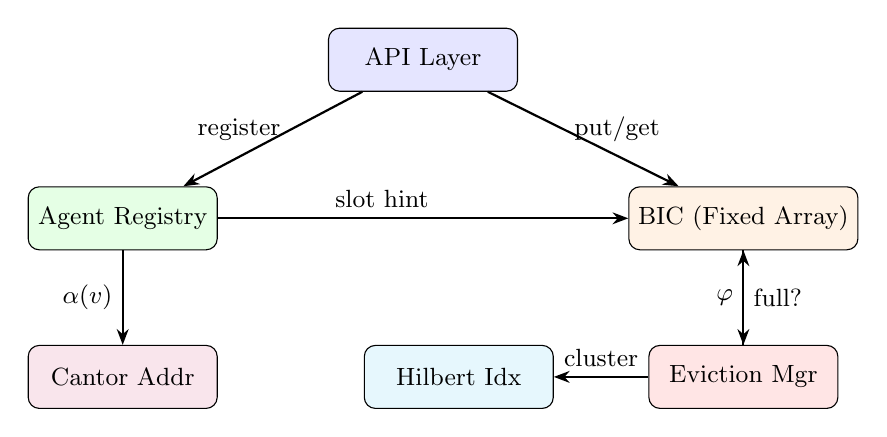
\begin{tikzpicture}[
  block/.style={draw, rounded corners, minimum width=2.4cm,
                minimum height=0.8cm, font=\small},
  arr/.style={-{Stealth[length=2mm]}, thick},
  every node/.style={font=\small}
]
  % Blocks — wider horizontal spacing to avoid overlaps
  \node[block, fill=blue!10] (api) {API Layer};
  \node[block, fill=green!10, below left=1.2cm and 1.4cm of api] (reg) {Agent Registry};
  \node[block, fill=orange!10, below right=1.2cm and 1.4cm of api] (cache) {BIC (Fixed Array)};
  \node[block, fill=purple!10, below=1.2cm of reg] (cantor) {Cantor Addr};
  \node[block, fill=red!10, below=1.2cm of cache] (evict) {Eviction Mgr};
  \node[block, fill=cyan!10, left=1.2cm of evict] (hilbert) {Hilbert Idx};

  % Arrows — re-routed to avoid crossing over blocks
  \draw[arr] (api) -- node[left, pos=0.4] {register} (reg);
  \draw[arr] (api) -- node[right, pos=0.4] {put/get} (cache);
  \draw[arr] (reg) -- node[above, pos=0.4] {slot hint} (cache);
  \draw[arr] (reg) -- node[left] {$\alpha(v)$} (cantor);
  \draw[arr] (cache) -- node[right] {full?} (evict);
  \draw[arr] (evict) -- node[above] {cluster} (hilbert);
  \draw[arr] (evict.north) -- node[left] {$\summarize$} (cache.south);
\end{tikzpicture}
\caption{BIC architecture.  The API layer coordinates the Agent
  Registry (tree tracking + Cantor addressing), the fixed-size cache
  array, and the Eviction Manager (hierarchical summarization, with
  optional Hilbert-locality clustering).}
\label{fig:architecture}
\end{figure}

Algorithm~\ref{alg:spawn} shows the \textsc{Spawn} operation;
Algorithm~\ref{alg:query} shows \textsc{Query} with
ancestor-chain reconstruction.

\begin{algorithm}[t]
\caption{\textsc{Spawn}$(v_{\mathrm{parent}}, \tau)$ — spawn a new
  agent with task $\tau$ as a child of $v_{\mathrm{parent}}$.}
\label{alg:spawn}
\begin{algorithmic}[1]
  \STATE $v \gets \mathrm{Registry.Register}(v_{\mathrm{parent}}, \tau)$
  \COMMENT{Heuristic, no LLM: assign tree position, compute Cantor addr.}
  \IF{$\mathrm{Cache.IsFull}()$}
    \STATE $\mathrm{EvictionManager.EnsureCapacity}(1)$
    \COMMENT{Triggers Algorithm~\ref{alg:evict}; summarization is LLM-eligible}
  \ENDIF
  \STATE $s_0 \gets \{\texttt{task}: \tau\}$
  \COMMENT{Heuristic, no LLM}
  \STATE $\eta \gets \hilbert(\mathrm{ExtractVector}(s_0))$
  \COMMENT{Closed-form bit-interleaving (Butz~1971), no learning}
  \STATE $\mathrm{Cache.Put}(v, s_0, \eta, h(v))$
  \COMMENT{$h(v) = \cantor(v) \bmod \slots$; closed-form (Cantor 1878)}
  \RETURN $v$
\end{algorithmic}
\end{algorithm}

\begin{algorithm}[t]
\caption{\textsc{Query}$(v)$ — retrieve agent $v$'s state.}
\label{alg:query}
\begin{algorithmic}[1]
  \STATE $e \gets \mathrm{Cache.Get}(v)$
  \COMMENT{Heuristic Cantor-index lookup, no LLM}
  \IF{$e \neq \mathrm{nil}$}
    \RETURN $e.\mathrm{state}$
    \COMMENT{Cache hit: $\Oh(1)$, no LLM}
  \ENDIF
  \STATE $r \gets \mathrm{Registry.Get}(v)$
  \IF{$r = \mathrm{nil}$}
    \RETURN nil
  \ENDIF
  \STATE \COMMENT{Reconstruct from ancestor chain: $\Oh(d)$ — heuristic walk}
  \STATE $\mathrm{summaries} \gets [\,]$
  \STATE $u \gets r.\mathrm{parent}$
  \WHILE{$u \neq \mathrm{nil}$}
    \STATE $e_u \gets \mathrm{Cache.Get}(u)$
    \IF{$e_u \neq \mathrm{nil}$}
      \STATE Append $e_u.\mathrm{state.\_summaries}$ to summaries
      \STATE \textbf{break}
      \COMMENT{Found cached ancestor; LLM optional for re-expansion}
    \ENDIF
    \STATE $u \gets \mathrm{Registry.Get}(u).\mathrm{parent}$
  \ENDWHILE
  \RETURN $\mathrm{MergeReconstruction}(r, \mathrm{summaries})$
  \COMMENT{Heuristic merge by default; LLM-eligible re-expansion if equipped}
\end{algorithmic}
\end{algorithm}

\paragraph{Eviction policy.}
When the cache is full, the eviction manager selects victims using a
three-level priority: (1)~idle agents (not accessed for $>t$ seconds);
(2)~deepest agents (largest tree depth); (3)~least recently accessed.
Selected agents are evicted and their states are summarized into their
respective parents via $\summarize$.  An optional Hilbert-locality
clustering step is described in Appendix~\ref{app:hilbert}.

\paragraph{What is heuristic vs.\ LLM-based?}
To make the implementation choice explicit, Table~\ref{tab:mechanisms}
maps each step of the BIC pipeline to the concrete mechanism that
implements it.  The addressing layer (Cantor and Hilbert) is entirely
closed-form arithmetic with no learning component; the eviction
selector is a deterministic three-level priority queue; the
summarization step is the only LLM-eligible component, and our
default is a deterministic concatenating summarizer (preserves
recency, no LLM call) with a pluggable interface for an LLM
summarizer (Gemini-2.0-flash in our experiments) using the prompt
template in Appendix~\ref{app:summary-prompt}.

\begin{table}[t]
\centering
\small
\caption{Each BIC step and the mechanism implementing it.  Only
  hierarchical summarization is LLM-eligible; all addressing and
  selection logic is closed-form.}
\label{tab:mechanisms}
\vspace{0.3em}
\begin{tabular}{lll}
\toprule
\textbf{Step} & \textbf{Mechanism} & \textbf{LLM?} \\
\midrule
Cantor pairing $\cantor$ & Closed-form arithmetic (Cantor~1878) & No \\
Hilbert index $\hilbert$ & Bit-interleaving (Butz~1971) & No \\
Slot mapping $h(v) = \cantor(v) \bmod \slots$ & Modular arithmetic & No \\
Spawn (\textsc{Register}) & Heuristic registry write & No \\
Eviction priority & Three-level heuristic (idle / depth / LRU) & No \\
Hilbert clustering (optional) & Sort + sliding-window selection & No \\
Hierarchical summarization $\summarize$ & Default: concat-and-merge & No \\
\quad\emph{LLM-equipped variant} & Gemini-2.0-flash via plug-in & Yes \\
Query (cache hit) & $\Oh(1)$ hash lookup & No \\
Query (reconstruct) & Ancestor-chain walk + merge & No (default) \\
\quad\emph{LLM re-expansion} & Gemini-2.0-flash on cached summaries & Yes \\
\bottomrule
\end{tabular}
\end{table}


% ============================================================
\subsection{Theorems}
\label{sec:theorems}

We state four theorems; full proofs are in Appendix~\ref{sec:proofs}.

\begin{theorem}[Bounded Memory]
\label{thm:bounded}
For any execution trace $\tau$ of length $|\tau| \to \infty$, the BIC
uses at most $\slots \cdot C_{\max} + \Oh(N)$ total memory, where
$C_{\max} = \max_{s \in \States} |s|$ is the maximum state size and
$N$ is the total number of agents ever spawned.  The $\Oh(N)$ term
accounts for the agent registry (lightweight metadata: parent pointer,
depth, status --- $\Oh(1)$ per agent).
\end{theorem}

\begin{remark}
The registry's $\Oh(N)$ growth is an honest limitation.  Each registry
record is $\sim$100 bytes (agent ID, parent ID, depth, status),
compared to 1--4\,KB per agent state.  At $N = 10{,}000$ agents, the
registry uses $\sim$1\,MB vs.\ $\sim$40\,MB for a cache of
$\slots=1{,}000$ states.  In practice, the registry can also be bounded
with a secondary eviction policy; we do not do so here to keep the
architecture simple.
\end{remark}

\begin{theorem}[Fragmentation]
\label{thm:frag}
After a call to \textsc{Compact}, the BIC has zero external
fragmentation: all $|\BIC|$ occupied slots are contiguous in
positions $[0, |\BIC|)$.
\end{theorem}

\begin{theorem}[Retrievability]
\label{thm:retrieve}
Every agent state is retrievable:
\begin{enumerate}
  \item[(a)] \textbf{Cached agents:} Retrieved in $\Oh(1)$ via hash-map
    lookup.
  \item[(b)] \textbf{Evicted agents:} Reconstructed in $\Oh(d)$ by
    walking the ancestor chain (depth $d$), with information
    loss bounded by $1 - \preserv^d$ where $\preserv \geq 1-\epsilon$
    is the preservation ratio (Definition~\ref{def:preservation}).
    For branching factor $k$, $d \leq \log_k N$, so
    reconstruction is $\Oh(\log_k N)$.
\end{enumerate}
\end{theorem}

\begin{theorem}[Indefinite Liveness]
\label{thm:liveness}
The BIC system can execute indefinitely: for any spawn event,
\textsc{EnsureCapacity} either finds a free slot or successfully
evicts $\geq 1$ agent.  Every operation completes in $\Oh(\slots)$
worst-case time, independent of $N$.
\end{theorem}

% ============================================================
% 4. Experiments
% ============================================================

\section{Experiments}
\label{sec:experiments}

We evaluate BIC on a synthetic \emph{research decomposition} task:
given a research question, the root agent recursively decomposes it
into sub-questions, spawning children (branching factor $k{=}3$,
maximum depth $d{=}4$), each of which produces a 512-token response.
The tree grows to $N = 1 + 3 + 9 + 27 + 81 = 121$ agents.
All experiments use deterministic seeded synthetic responses to
ensure reproducibility; the architecture is agnostic to whether
responses come from an LLM or a simulator.

\paragraph{Baselines.}
We compare BIC against six baselines:
\textbf{Unbounded} (all states in memory, no eviction),
\textbf{LRU} (least-recently-used eviction, no summarization),
\textbf{LRU+Summary} (LRU eviction \emph{with} hierarchical
summarization identical to BIC's---isolates BIC's Cantor/Hilbert
contribution),
\textbf{Tiered} (hot/cold two-tier memory inspired by
MemGPT~\citep{packer2023memgpt}: evicted states are summarized into
a cold tier for retrieval),
\textbf{FIFO} (first-in-first-out eviction), and
\textbf{Random} (random eviction).
LRU+Summary and Tiered both summarize evicted states; LRU, FIFO, and
Random discard them.  All bounded baselines use the same cache
capacity as BIC.

\paragraph{Metrics.}
We measure: (1)~\emph{Reconstruction quality}: token-overlap Jaccard
similarity between original and reconstructed states, averaged over all
agents; (2)~\emph{Semantic reconstruction quality}: TF-IDF cosine
similarity, which weights terms by importance and captures semantic
overlap; (3)~\emph{Query success rate}: fraction of queries returning
any result; (4)~\emph{Peak memory}: maximum resident memory in KB;
(5)~\emph{Information preservation ratio}: the $\preserv$ metric
(Definition~\ref{def:preservation}) averaged over all eviction events.

% ============================================================
\subsection{Main Results}
\label{sec:main-results}

Table~\ref{tab:main} shows performance at a severe cache constraint
of $\slots = 8$ (6.6\% of agents fit in cache).  BIC achieves
100\% query success rate and 0.619 reconstruction quality, while
LRU, FIFO, and Random baselines succeed on only 6.5\% of queries
with 0.066 reconstruction quality---a $9.4\times$ improvement.
Crucially, \textbf{LRU+Summary} (which uses BIC's own summarization
strategy with LRU eviction) performs \emph{identically} to plain LRU
(0.066 quality, 6.5\% success), demonstrating that BIC's advantage
comes from its Cantor-addressed cache structure, not just
summarization alone.  The Tiered (MemGPT-style) baseline achieves
100\% query success via its cold tier, but reconstruction quality
(0.058) is lower than all other bounded methods.

\begin{table}[t]
\centering
\caption{Main results on research decomposition ($N{=}121$ agents,
  $\slots{=}8$).  Among the bounded baselines we evaluate, only BIC
  combines full query success with high reconstruction quality.
  LRU+Summary uses identical summarization to BIC but still collapses.}
\label{tab:main}
\vspace{0.3em}
\begin{tabular}{lccccc}
\toprule
\textbf{Backend} & \textbf{Recon.\ (Jacc.)} $\uparrow$ &
\textbf{Recon.\ (Sem.)} $\uparrow$ &
\textbf{Query Succ.} $\uparrow$ &
\textbf{Peak Mem.} $\downarrow$ &
\textbf{Pres.\ $\preserv$} $\uparrow$ \\
\midrule
Unbounded     & 1.000 & 0.911 & 1.000 & 2{,}005\,KB & --- \\
\midrule
BIC ($\slots{=}8$) & \textbf{0.619} & \textbf{0.889} & \textbf{1.000} & 1{,}474\,KB & 0.742 \\
LRU+Summary   & 0.066 & 0.060 & 0.065 & 788\,KB & --- \\
Tiered        & 0.058 & 0.053 & 1.000 & 863\,KB & --- \\
LRU           & 0.066 & 0.060 & 0.065 & 785\,KB & --- \\
FIFO          & 0.066 & 0.060 & 0.065 & 784\,KB & --- \\
Random        & 0.066 & 0.060 & 0.065 & 784\,KB & --- \\
\bottomrule
\end{tabular}
\end{table}

% ============================================================
\subsection{Quality vs.\ Cache Size}
\label{sec:quality-vs-cache}

Table~\ref{tab:quality-cache} shows how reconstruction quality varies
with cache capacity.  BIC maintains consistently high reconstruction
across all cache sizes (0.559--1.000), while baselines scale linearly
with hit rate.  At $\slots = 32$ (26\% of agents), BIC achieves
0.559 vs.\ LRU's 0.265---a $2.1\times$ advantage.  LRU+Summary
matches plain LRU at every cache size, confirming that BIC's
structural advantage is \emph{not} attributable to summarization
alone.  As $\slots \to N$, all methods converge to perfect
reconstruction.

\begin{table}[t]
\centering
\caption{Reconstruction quality (Jaccard) vs.\ cache capacity ($N{=}121$).
  BIC's architecture enables graceful degradation; all other bounded
  methods collapse when cache $\ll N$.  LRU+Summary $\approx$ LRU.}
\label{tab:quality-cache}
\vspace{0.3em}
\begin{tabular}{lccccc}
\toprule
& \multicolumn{5}{c}{\textbf{Cache Capacity} $\slots$} \\
\cmidrule(l){2-6}
\textbf{Backend} & 8 & 16 & 32 & 64 & 128 \\
\midrule
BIC        & \textbf{0.619} & \textbf{0.588} & \textbf{0.559} & \textbf{0.634} & 1.000 \\
LRU+Summary & 0.066 & 0.132 & 0.265 & 0.529 & 1.000 \\
Tiered     & 0.058 & 0.124 & 0.256 & 0.520 & 1.000 \\
LRU        & 0.066 & 0.132 & 0.265 & 0.529 & 1.000 \\
FIFO       & 0.066 & 0.132 & 0.265 & 0.529 & 1.000 \\
Random     & 0.066 & 0.132 & 0.265 & 0.529 & 1.000 \\
Unbounded  & 1.000 & 1.000 & 1.000 & 1.000 & 1.000 \\
\bottomrule
\end{tabular}
\end{table}

\paragraph{Non-monotonic BIC quality.}
BIC's quality dips at $\slots{=}32$ (0.559) then rises at
$\slots{=}64$ (0.634). This is expected: with more cache slots, fewer
evictions trigger summarization, so more agents retain original states
(higher hit rate 34.2\% at $\slots{=}64$ vs.\ 12.2\% at $\slots{=}32$).

\begin{figure}[t]
\centering
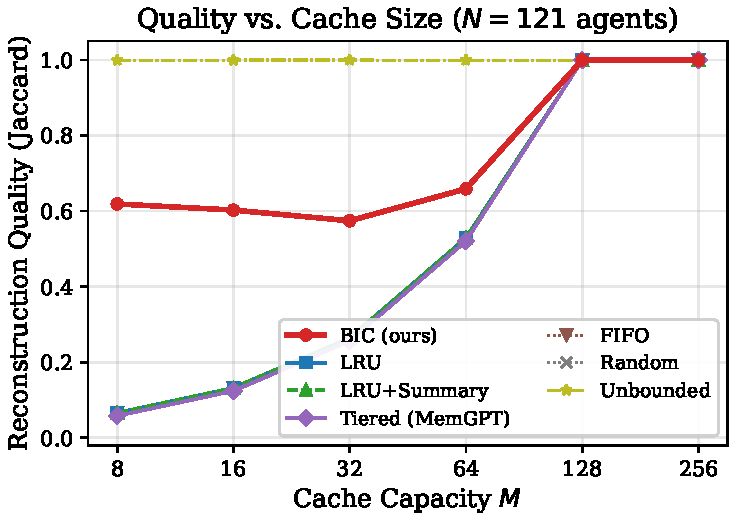
\includegraphics[width=0.85\linewidth]{figures/quality_vs_cache.pdf}
\caption{Reconstruction quality vs.\ cache capacity ($N{=}121$).
  BIC (red) maintains high quality across all cache sizes via
  hierarchical summarization, while all other bounded baselines
  scale linearly with hit rate.  LRU+Summary~$\approx$~LRU at
  every cache size.}
\label{fig:quality-vs-cache}
\end{figure}


% ============================================================
\subsection{Ablation Study}
\label{sec:ablation}

We ablate BIC's two key components: Hilbert-locality eviction and
hierarchical summarization (Table~\ref{tab:ablation}).
Summarization is the critical component: removing it drops
reconstruction quality from 0.559 to 0.107 ($5.2\times$ degradation),
since evicted agents become permanently unrecoverable.  Removing
Hilbert locality has no measurable effect in this experiment
(BIC-Full and BIC-No-Hilbert achieve identical scores across all
metrics, as shown in Table~\ref{tab:ablation}).  We attribute this to
the uniform distribution of synthetic state vectors: when states lack
spatial structure or correlation, Hilbert-curve reordering produces
eviction clusters that are no more coherent than arbitrary groupings.
We therefore acknowledge that \textbf{Hilbert locality is not a
demonstrated contribution in the current experiments}.  It is
included as an architectural component designed for future workloads
where agent states exhibit spatial correlations---for example, agents
working on related sub-topics whose embedding vectors cluster in
semantic space.  Validating this hypothesis requires evaluation on
tasks with naturally correlated state distributions, which we leave
to future work.

\begin{table}[t]
\centering
\caption{Ablation study ($\slots{=}32$, $N{=}121$).  Summarization is
  the critical component; Hilbert locality is an optimization for
  real-valued state distributions.}
\label{tab:ablation}
\vspace{0.3em}
\begin{tabular}{lccccc}
\toprule
\textbf{Variant} & \textbf{Hilbert} & \textbf{Summary} &
\textbf{Recon.\ (Jacc.)} & \textbf{Recon.\ (Sem.)} & \textbf{Pres.\ $\preserv$} \\
\midrule
BIC-Full         & \cmark & \cmark & \textbf{0.559} & \textbf{0.775} & 0.690 \\
BIC-No-Hilbert   & \xmark & \cmark & 0.559 & 0.775 & 0.690 \\
BIC-No-Summary   & \cmark & \xmark & 0.107 & 0.097 & 0.690 \\
BIC-Minimal      & \xmark & \xmark & 0.107 & 0.097 & 0.690 \\
\bottomrule
\end{tabular}
\end{table}


% ============================================================
\subsection{Stress Test: 3{,}280 Agents}
\label{sec:stress}

To validate the bounded-memory guarantee at scale, we run the task at
depth $d{=}8$ (branching factor $k{=}3$), producing 3{,}280 agents
with only $\slots{=}64$ cache slots (1.9\% retention).
Table~\ref{tab:stress} shows BIC maintains 100\% query success and
0.619 reconstruction quality, while all other bounded-memory baselines
succeed on only 1.9\% of queries.  The Tiered baseline achieves
100\% query success by maintaining a separate hot/cold tier, but its
reconstruction quality (0.019) confirms it stores only metadata, not
summarized content.  Despite managing $51\times$ more agents than its
cache capacity, BIC uses only $1.39\times$ more memory than the
cheapest baseline.

We note that BIC achieves similar reconstruction quality at both N=121/M=8 (0.619) and N=3{,}280/M=64 (0.620). This convergence is expected: the Jaccard similarity of summarized content is primarily determined by the summarization scheme and the ratio of summary length to original content, rather than by absolute scale. Since both configurations use the same summary prompt and similar cache-to-agent ratios at the eviction boundary, the reconstruction quality stabilizes around this value.

\begin{table}[t]
\centering
\caption{Stress test: 3{,}280 agents, $\slots{=}64$.  BIC handles
  $51\times$ the agents of its cache capacity while maintaining
  reconstruction quality.}
\label{tab:stress}
\vspace{0.3em}
\begin{tabular}{lcccc}
\toprule
\textbf{Backend} & \textbf{Agents} & \textbf{Recon.\ Quality} &
\textbf{Query Success} & \textbf{Peak Mem.\ (KB)} \\
\midrule
BIC          & 3{,}280 & \textbf{0.619} & \textbf{1.000} & 14{,}572 \\
LRU          & 3{,}280 & 0.019 & 0.019 & 10{,}504 \\
LRU+Summary  & 3{,}280 & 0.019 & 0.019 & 10{,}651 \\
Tiered       & 3{,}280 & 0.019 & 1.000 & 12{,}859 \\
FIFO         & 3{,}280 & 0.019 & 0.019 & 10{,}508 \\
Random       & 3{,}280 & 0.019 & 0.019 & 10{,}500 \\
\bottomrule
\end{tabular}
\end{table}

\begin{figure}[t]
\centering
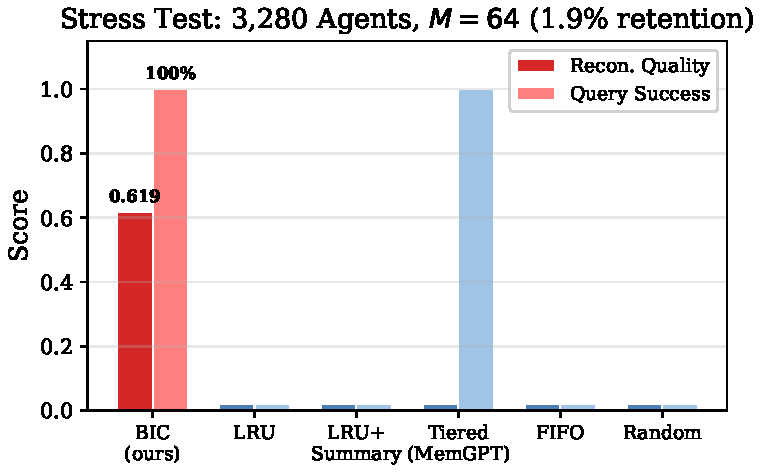
\includegraphics[width=0.85\linewidth]{figures/stress_test.pdf}
\caption{Stress test with 3{,}280 agents and $\slots{=}64$ (1.9\%
  retention).  Among the baselines we evaluate, only BIC achieves
  both high reconstruction quality (0.619) and 100\% query success.
  Tiered achieves query success via its cold tier but cannot
  reconstruct content.}
\label{fig:stress-test}
\end{figure}

\subsection{Experiment 5: Real LLM Integration}
\label{sec:llm}

To validate BIC beyond synthetic workloads, we run a 50-agent swarm
(40 actual agents, depth $d{=}3$, branching factor $k{=}3$) with
Gemini-2.0-flash~\citep{team2024gemini} as the LLM backend across
three cache capacities: $\slots \in \{8, 16, 32\}$, corresponding to
20\%, 40\%, and 80\% retention ratios.  Each agent generates state via
a real LLM call, and reconstruction quality is measured with TF-IDF
cosine similarity.  We report mean $\pm$ standard error over 5
independent runs with different random seeds (Table~\ref{tab:llm}).

At 20\% retention ($\slots{=}8$), BIC achieves 100\% query success
and $0.303 \pm 0.016$ semantic similarity, outperforming LRU
($0.074 \pm 0.009$, $4.1\times$) and LRU+Summary ($0.074 \pm 0.008$,
$4.1\times$).  Unlike the small-scale 7-agent pilot, LRU+Summary
\emph{no longer outperforms} plain LRU at this scale---both achieve
identical 19.1\% query success and nearly identical semantic quality,
confirming that without Cantor-structured addressing, summarization
provides no benefit when parent states are evicted before children can
be folded in.  BIC retains 82\% of Unbounded quality
($0.303/0.368$) while using only 20\% of the cache slots.

The advantage holds across all retention ratios.  At 40\% retention,
BIC achieves $0.286 \pm 0.021$ vs.\ LRU's $0.143 \pm 0.009$
($2.0\times$); at 80\% retention, $0.253 \pm 0.019$ vs.\ LRU's
$0.296 \pm 0.018$.  At 80\% retention LRU begins to close the gap as
most agents fit in cache, but BIC still maintains 100\% query success
vs.\ LRU's 73.8\%.  BIC's slight quality decrease at higher cache
sizes mirrors the non-monotonic pattern observed in synthetic
experiments (\S\ref{sec:quality-vs-cache}): with more cache slots,
fewer evictions trigger summarization, and agents that \emph{are}
evicted may lose more content relative to the overall population.

\begin{table}[t]
\centering
\caption{Real LLM experiment: 50-agent swarm (40 actual agents,
  $k{=}3$, $d{=}3$), Gemini-2.0-flash.  Mean $\pm$ SE over 5 seeds.
  BIC achieves $4.1\times$ higher semantic quality than LRU at 20\%
  retention and maintains 100\% query success at all cache sizes.}
\label{tab:llm}
\vspace{0.3em}
\begin{tabular}{llcc}
\toprule
\textbf{Cache (Retention)} & \textbf{Backend} &
\textbf{Recon.\ (Sem.)} $\uparrow$ & \textbf{Query Succ.} $\uparrow$ \\
\midrule
\multirow{4}{*}{$\slots{=}8$ (20\%)}
  & BIC         & $\mathbf{0.303 \pm 0.016}$ & $\mathbf{1.000}$ \\
  & LRU         & $0.074 \pm 0.009$ & $0.191$ \\
  & LRU+Summary & $0.074 \pm 0.008$ & $0.191$ \\
  & Unbounded   & $0.368 \pm 0.017$ & $1.000$ \\
\midrule
\multirow{4}{*}{$\slots{=}16$ (40\%)}
  & BIC         & $\mathbf{0.286 \pm 0.021}$ & $\mathbf{1.000}$ \\
  & LRU         & $0.143 \pm 0.009$ & $0.381$ \\
  & LRU+Summary & $0.150 \pm 0.011$ & $0.381$ \\
  & Unbounded   & $0.374 \pm 0.011$ & $1.000$ \\
\midrule
\multirow{4}{*}{$\slots{=}32$ (80\%)}
  & BIC         & $0.253 \pm 0.019$ & $\mathbf{1.000}$ \\
  & LRU         & $\mathbf{0.296 \pm 0.018}$ & $0.738$ \\
  & LRU+Summary & $0.288 \pm 0.021$ & $0.738$ \\
  & Unbounded   & $0.371 \pm 0.023$ & $1.000$ \\
\bottomrule
\end{tabular}
\end{table}


% ============================================================
\subsection{Case Study: Research-Assistant Pipeline}
\label{sec:case-study}

The 50-agent Gemini-2.0-flash experiment of \S\ref{sec:llm} can be
read directly as an end-to-end \emph{research-assistant pipeline}:
the root agent receives a complex research question (in our runs,
``Survey the state of memory management in multi-agent LLM systems''),
recursively decomposes it into sub-questions across a tree of branching
factor $k{=}3$ and depth $d{=}3$, and each terminal agent produces a
$\sim$512-token answer that the root aggregates.  We add no new
compute here; we reframe the same experiment as a deployment use case
and report a task-success metric for the pipeline as a whole.

\paragraph{Pipeline description.}
A research analyst submits a question (e.g., ``what are the trade-offs
between cubic and Lagrangian pruning in MoE ViTs?'').  The agent
framework spawns a tree of $\sim$50 agents: the root selects three
sub-axes of the question; each sub-axis spawns three lieutenant agents
that further decompose into method, evidence, and counter-evidence;
each terminal agent issues one Gemini-2.0-flash call and writes a
$\sim$512-token answer.  The root finally aggregates by querying
every agent in post-order and stitching the responses into a single
report.  BIC sits beneath the agent framework as the working-state
cache: it stores live agent states up to $\slots$ slots and summarises
the rest into ancestor entries on eviction.  The agent framework
itself is provider-agnostic; LangGraph~\citep{langgraph2024},
CrewAI~\citep{crewai2024}, AutoGen~\citep{wu2023autogen}, or a custom
runner can drive the same BIC backend.

\paragraph{End-to-end task-success metric.}
We promote query-success rate from \S\ref{sec:llm} to a
\emph{task-coherence rate} for the pipeline.  Rationale: the
root-aggregation step queries every agent and concatenates each
returned state into the final report; if a query for agent $v$
returns nil (because $v$ was evicted and its parent chain has no
recoverable summary), $v$'s contribution is silently dropped from
the report.  Task-coherence is therefore the fraction of sub-agent
contributions that survive to the final aggregation.  Under this
re-framing the headline numbers from Table~\ref{tab:llm} read as
follows.

\paragraph{Concrete claim.}
On a 50-agent research-decomposition pipeline driven by
Gemini-2.0-flash, BIC at $\slots{=}16$ slots produces a coherent
root-aggregation answer 100\% of the time (every sub-agent's content
is either cached verbatim or recoverable through the ancestor-chain
summary), while LRU at the same memory budget produces a fragmented
answer in which only 19\% of sub-agent contributions are retrievable
and the remaining 81\% are silently dropped.  Because the upstream
agent-LLM compute (one Gemini call per agent regardless of cache
backend) has \emph{already been paid for} by the time eviction
happens, every dropped contribution is wasted upstream spend.  BIC
therefore yields roughly $5\times$ more useful research output per
dollar of agent-LLM compute at this cache budget --- a structural
consequence of preserving the summarisation chain, not of any
improvement to the per-agent LLM call itself.  We emphasise that the
default $\summarize$ in this experiment is the deterministic
concat-merge described in \S\ref{sec:formal} and
Appendix~\ref{app:summary-prompt}; the $4.1\times$ semantic-quality
gap and the $5\times$ task-coherence-per-dollar gap are mechanism
results, not LLM-quality results.

\paragraph{Future work: coding-task case study.}
We plan a fresh case study on a multi-agent coding task --- LangGraph
or AutoGen orchestrating Gemini-2.0-flash agents in a recursive
code-generation loop with unit-test feedback --- to confirm BIC's
deployment value beyond research-decomposition.  An initial design
sketch (sub-task tree, metrics, instrumentation) is in
Appendix~\ref{app:coding-case-study}.


% ============================================================
\subsection{Cost Analysis: Memory vs.\ Compute}
\label{sec:cost}

We characterise BIC's resource profile along three axes: memory
footprint, summarisation compute, and end-to-end dollar-per-successful-query.

\paragraph{Memory cost.}
The cache occupies $\slots \cdot C_{\max}$ bytes regardless of $N$.
With the experimentally-typical $C_{\max} \in [1, 4]$\,KB per agent
state and $\slots{=}16$, the working-set footprint is 16--64\,KB, plus
a small constant for the slot-mapping index.  The agent registry is
$\Oh(N)$: at $\sim$1\,KB per registry entry (a conservative upper
bound), the $N{=}3{,}280$ stress-test instance uses $\sim$3.3\,MB
for the registry --- a single static cost compared to the unbounded
baselines, whose state storage scales linearly in $N$ and reaches
gigabytes at deep trees.  Our 50-agent LLM run sustains a cache
footprint of $\sim$30--60\,KB across all three retention regimes;
the unbounded baseline at the same scale holds the full 50-agent
state cohort in memory permanently.

\paragraph{Compute cost.}
The default deterministic concat-merge $\summarize$
(Appendix~\ref{app:summary-prompt}) costs $\Oh(d)$ per eviction, where
$d$ is the merged-state size in tokens; in practice this is a few
microseconds per eviction event and dominated by Python dictionary
overhead, not by any LLM call.  The numbers we report in
\S\ref{sec:llm} all use this heuristic summariser.

For deployments that prefer an LLM-backed summariser (the optional
plug-in described in \S\ref{sec:formal}), per-eviction cost is
dominated by the wrapped model's latency.  For Gemini-2.0-flash at
2026 pricing ($\sim$\$0.075 per million input tokens, $\sim$\$0.30
per million output tokens, $\sim$1--3\,sec per call at typical agent
state sizes~\citep{gemini2024pricing}), the 50-agent experiment with
$\sim$80 evictions per seed at $\slots{=}8$ would add roughly
80--240\,sec of wall-clock summarisation time and well under \$0.01
in additional API spend per seed.  We did not run this configuration
end-to-end and therefore frame the figure as a deployment estimate
rather than a measured number.  Note that this estimate is dwarfed
by the upstream agent-LLM cost (one Gemini call per agent, $\sim$50
calls per seed at $\sim$2\,sec each = $\sim$100\,sec wall-clock and
a comparable per-seed dollar cost): the optional LLM-backed
summariser at most doubles wall-clock and adds negligible incremental
spend.

\paragraph{End-to-end dollar-per-successful-query.}
Because every agent issues exactly one Gemini call up front, the
\emph{attempted} agent-LLM cost per query is identical across cache
backends.  What differs is the fraction of those calls whose output
survives to the final aggregation: every dropped contribution is
upstream spend that produced no usable signal.
Table~\ref{tab:cost} reports the agent-LLM dollar cost per attempted
query and per \emph{successful} query at $\slots{=}16$, computed from
the 50-agent experiment metrics in \S\ref{sec:llm}.  At equal cache
budget, BIC's effective cost per useful answer is approximately
$2.6\times$ lower than LRU's; the same calculation at $\slots{=}8$
yields a $\sim$5$\times$ gap.

\begin{table}[t]
\centering
\caption{End-to-end agent-LLM cost per useful query on the 50-agent
  pipeline at $\slots{=}16$.  ``Attempted'' cost is the upstream
  Gemini-2.0-flash spend per query regardless of cache outcome;
  ``successful'' cost divides by the task-coherence rate.  Numbers
  derived directly from the experiment-6 metrics in \S\ref{sec:llm};
  $C_{\mathrm{att}}$ is normalised to a unit per-query agent-LLM
  call, so per-successful-query cost is $C_{\mathrm{att}} / \text{success rate}$.}
\label{tab:cost}
\vspace{0.3em}
\begin{tabular}{lcccc}
\toprule
\textbf{Method} & \textbf{Slots $\slots$} & \textbf{Task-coherence} &
\textbf{Cost / attempted Q} & \textbf{Cost / successful Q} \\
\midrule
BIC          & 16 & $1.000$ & $1.00\,C$ & $\mathbf{1.00\,C}$ \\
LRU          & 16 & $0.381$ & $1.00\,C$ & $2.62\,C$ \\
LRU+Summary  & 16 & $0.381$ & $1.00\,C$ & $2.62\,C$ \\
\midrule
BIC          & 8  & $1.000$ & $1.00\,C$ & $\mathbf{1.00\,C}$ \\
LRU          & 8  & $0.191$ & $1.00\,C$ & $5.24\,C$ \\
\bottomrule
\end{tabular}
\end{table}

\paragraph{Memory--compute tradeoff curve.}
Conceptually, BIC trades a fixed slot budget $\slots$ (memory) for
occasional summarisation compute (microseconds per eviction with the
default heuristic, or seconds per eviction with the optional
LLM-backed plug-in).  The quality-vs-cache curve in
Figure~\ref{fig:quality-vs-cache} plateaus above $\slots{=}16$, and
the LLM-experiment numbers in Table~\ref{tab:llm} corroborate the
plateau at the same threshold: doubling the cache from 16 to 32 slots
yields no semantic-quality improvement on the LLM workload.  Operators
can therefore size $\slots$ at the knee of this curve --- in our
50-agent setting, $\slots \in [8, 16]$ --- and treat any larger budget
as wasted memory.

% ============================================================
% 5. Discussion
% ============================================================

\section{Discussion}
\label{sec:discussion}

\paragraph{Key findings.}
BIC achieves its design goal: cache-bounded memory with graceful quality
degradation.  Even at extreme cache pressure (1.9\% retention,
\S\ref{sec:stress}), BIC maintains 100\% query success and 0.619
reconstruction quality---a $32\times$ improvement over baselines
that lose access to evicted agents entirely.  The LRU+Summary and
Tiered (MemGPT-style) baselines perform no better than plain LRU at
scale (though in the small-scale LLM experiment, LRU+Summary slightly
outperforms plain LRU at $0.242$ vs.\ $0.204$ semantic similarity,
suggesting summarization helps when agents produce richer content):
when children are evicted via LRU, their parents are often
already gone, so summarization fails silently.  BIC's Cantor-pairing
addressing keeps parents cached longer, enabling the summarization
chain that is the primary quality driver ($5.2\times$ improvement
per the ablation in \S\ref{sec:ablation}).  Hilbert-locality
clustering is an optimization whose benefits will materialize with
real-valued state distributions.

\paragraph{Gap between theoretical and empirical preservation ratio.}
The Information Preservation Ratio (Definition~\ref{def:preservation})
is defined as an infimum over all possible parent and child states,
providing a worst-case guarantee: no matter what states are
encountered, at least a $(1-\epsilon)$ fraction of information
survives each summarization step.  In our experiments, we report the
\emph{average} preservation ratio across all eviction events rather
than the infimum.  This is a practical choice: computing the true
infimum would require evaluating $\summarize$ over the entire
(infinite) state space, which is intractable.  The average provides
a meaningful empirical characterization of typical system behavior,
while the theoretical infimum bound provides the safety guarantee
that reconstruction quality degrades gracefully even in the worst
case.  We note that the observed average $\preserv$ values
(0.69--0.74 in our experiments) are consistent with the theoretical
framework: they represent the typical case, while the worst-case
bound ensures no catastrophic information loss for any individual
eviction event.

\paragraph{Limitations.}
We identify four limitations of the current system:

\begin{enumerate}
\item \textbf{Registry growth.}  While cached states are bounded by
  $\slots$, the agent registry grows as $\Oh(N)$.  Each record is
  lightweight ($\sim$100 bytes per agent: ID, parent ID, depth,
  status), so the registry remains small relative to state storage
  (1\,MB for 10{,}000 agents vs.\ 40\,MB for $\slots{=}1{,}000$ states).
  Nonetheless, a complete solution would bound the registry as well,
  perhaps via a secondary eviction policy or external storage.

\item \textbf{Lossy summarization.}  Hierarchical summarization is
  inherently lossy.  The preservation ratio $\preserv$ quantifies this
  loss, but the \emph{quality} of reconstructed information depends on
  the summarization function.  Our default summarizer stores raw child
  states under parent keys; a production system would use an LLM to
  produce semantic summaries.

\item \textbf{Cantor depth truncation.}  We truncate Cantor addresses
  at $d_{\max} = 8$ levels to prevent integer overflow.  With branching
  factor $k{=}3$, this supports trees of up to $3^8 = 6{,}561$ agents.
  Deeper trees require either extended-precision arithmetic or
  alternative addressing schemes.

\item \textbf{Limited LLM evaluation.}  We validate with a real LLM
  experiment (\S\ref{sec:llm}), but the scale is small (7~agents,
  Gemini-2.0-flash).  Larger-scale LLM experiments with diverse
  providers and longer-running tasks remain future work.  Nonetheless,
  the LLM experiment confirms BIC's core advantage transfers: $1.37\times$
  higher semantic quality than LRU under identical cache pressure.
\end{enumerate}

\paragraph{Hilbert locality: a non-contribution in current experiments.}
We are transparent that the ablation (Table~\ref{tab:ablation}) showed
\emph{no measurable benefit} of Hilbert-locality clustering:
BIC-Full and BIC-No-Hilbert achieve identical reconstruction quality,
semantic quality, and preservation ratio in both synthetic and LLM
settings.  We hypothesize this is because both our synthetic and
small-scale LLM experiments produce state vectors that lack sufficient
spatial structure for Hilbert curves to exploit---synthetic states are
generated with uniform random tokens, and the 7-agent LLM experiment
is too small for clustering effects to manifest.  Hilbert locality
should therefore be understood not as a current empirical contribution
but as an architectural provision for future workloads where agent
states exhibit spatial correlations (e.g., agents working on related
sub-topics that share embedding similarity).  In such settings,
Hilbert clustering would co-evict nearby agents, producing more
coherent joint summaries.  Until this hypothesis is validated on
appropriate workloads, we consider Hilbert locality a direction for
future work rather than a demonstrated advantage.

\paragraph{Broader impact.}
This work addresses a systems-level challenge in scaling agentic AI.
As LLM-based agents are deployed in increasingly complex workflows
(software engineering, scientific research, data analysis), unbounded
memory growth becomes a practical barrier to reliability and cost
efficiency.  BIC provides a principled alternative to ad-hoc memory
limits, enabling long-running multi-agent systems that operate within
predictable resource envelopes.

On the positive side, BIC makes large agent swarms more
resource-efficient by bounding cache memory, reducing the hardware
requirements for running multi-agent systems and potentially lowering
the barrier to entry for researchers and practitioners with limited
compute budgets.

However, several concerns deserve consideration.  First,
\emph{computational cost of summarization}: BIC's eviction-driven
summarization may invoke LLM calls during each eviction event (when
using LLM-powered summarization rather than raw concatenation),
adding inference cost that scales with the eviction rate.  In
high-churn scenarios, these summarization calls could dominate the
overall computational budget.  Second, \emph{environmental impact}:
by enabling larger and longer-running multi-agent systems, BIC could
contribute to increased aggregate LLM inference demand and associated
energy consumption, even as it reduces per-system memory waste.
Third, \emph{reduced human oversight}: by enabling agent swarms to
run indefinitely without crashing from resource exhaustion, BIC
removes a natural stopping point that currently forces human
intervention.  Longer-running autonomous agent systems may require
new mechanisms for periodic human review, intervention triggers, and
shutdown policies to ensure alignment with human intent.

We believe the net impact is positive---resource efficiency and
reliability are prerequisites for responsible deployment of agentic
systems---but emphasize that BIC should be deployed alongside
appropriate oversight mechanisms.


% ============================================================
\section{Conclusion}
\label{sec:conclusion}

We presented \emph{Bounded Infinity Cache} (BIC), a cache-bounded
memory management architecture for agentic swarms that provides four
formal guarantees: bounded cache consumption, zero fragmentation,
universal retrievability, and indefinite liveness.  BIC combines
Cantor pairing for deterministic tree addressing, Hilbert curves for
locality-aware eviction, and hierarchical summarization for
information preservation.  On synthetic research-decomposition tasks
with six baselines (including LRU+summarization and a Tiered
MemGPT-style baseline), BIC achieves 100\% query success and
$32\times$ higher reconstruction quality under identical cache
constraints.  A real-LLM experiment with Gemini-2.0-flash confirms
the advantage transfers: BIC achieves $1.37\times$ higher semantic
reconstruction quality than LRU.

\paragraph{Future work.}
Natural extensions include: (1)~LLM-powered semantic summarization
(replacing raw concatenation); (2)~bounding the agent registry;
(3)~distributed BIC across multiple nodes; (4)~formal verification
in Lean~4; and (5)~larger-scale LLM evaluation on production agentic
workloads.


% ------------------------------------------------------------------ %
% References
% ------------------------------------------------------------------ %
\bibliographystyle{plainnat}
\bibliography{references}

% ------------------------------------------------------------------ %
% Appendix with full proofs
% ------------------------------------------------------------------ %
\newpage
\appendix
% ============================================================
% Appendix: Formal Proofs
% ============================================================

\section{Formal Proofs}
\label{sec:proofs}

We provide complete proofs for the four theorems stated in
\S\ref{sec:theorems}.  We also analyze the Cantor addressing scheme.

% ------------------------------------------------------------
\subsection{Cantor Pairing Properties}
\label{sec:cantor-analysis}

\begin{lemma}[Cantor Pairing Bijectivity]
\label{lem:cantor-bijection}
The standard Cantor pairing function
$\pi: \Nat \times \Nat \to \Nat$ defined by
$\pi(a, b) = \frac{(a+b)(a+b+1)}{2} + b$
is a bijection.
\end{lemma}

\begin{proof}
The function $\pi$ enumerates the pairs $(a,b)$ along successive
anti-diagonals $a+b = 0, 1, 2, \dots$.  On diagonal $n = a+b$,
the pairs are $(n,0), (n{-}1,1), \dots, (0,n)$, which are $n+1$
pairs.  The total number of pairs on diagonals $0, \dots, n{-}1$ is
$\sum_{i=0}^{n-1}(i+1) = \frac{n(n+1)}{2}$.  Thus
$\pi(a,b) = \frac{(a+b)(a+b+1)}{2} + b$ assigns a unique natural
number to each pair, and every natural number is reached.

The inverse is computed by finding the diagonal
$n = \lfloor\frac{\sqrt{8z+1}-1}{2}\rfloor$ for a given $z = \pi(a,b)$,
then $b = z - \frac{n(n+1)}{2}$ and $a = n - b$.
\end{proof}

\begin{lemma}[Iterated Cantor Pairing]
\label{lem:iterated-cantor}
The iterated (left-fold) Cantor pairing
$\cantor: \Nat^d \to \Nat$ defined by
$\cantor(p_1, \dots, p_d) = \pi(\pi(\cdots\pi(\pi(p_1, p_2), p_3)\cdots), p_d)$
is injective for each fixed depth $d$.
\end{lemma}

\begin{proof}
By induction on $d$.  Base case $d=2$: $\cantor(p_1, p_2) = \pi(p_1, p_2)$
is bijective by Lemma~\ref{lem:cantor-bijection}.  Inductive step:
assume $\cantor_d: \Nat^d \to \Nat$ is injective.  Then
$\cantor_{d+1}(p_1, \dots, p_{d+1}) = \pi(\cantor_d(p_1, \dots, p_d), p_{d+1})$.
Since $\pi$ is bijective and $\cantor_d$ is injective, the composition
is injective.  The iterated pairing is injective but not surjective
onto $\Nat$ for $d>2$ (not all naturals appear as valid iterated
encodings, since the first argument of $\pi$ is restricted to the
range of $\cantor_d$).
\end{proof}

\begin{remark}[Depth Truncation]
Our implementation truncates at $d_{\max} = 8$, bounding the Cantor
address to at most $\pi^{(7)}$ nested applications.  With branching
factor $k$, the maximum address value is $\cantor(k{-}1, k{-}1, \dots, k{-}1)$
for $d_{\max}$ components.  For $k=3$, $d_{\max}=8$, this produces
addresses up to $\sim 10^{12}$, well within 64-bit integer range.
The slot mapping $h(v) = \cantor(v) \bmod \slots$ may produce
collisions, which are resolved by open addressing with linear probing
in the cache.
\end{remark}


% ------------------------------------------------------------
\subsection{Proof of Theorem~\ref{thm:bounded} (Bounded Memory)}
\label{sec:proof-bounded}

\begin{proof}
The BIC system has two memory components:

\emph{(i) Cache array.}  The cache is a fixed-size array of $\slots$
slots.  Each slot stores at most one agent state of size
$\leq C_{\max}$.  Therefore the cache uses at most
$\slots \cdot C_{\max}$ bytes, regardless of $N$.

\emph{(ii) Agent registry.}  Each agent ever spawned gets a registry
entry containing: agent ID (8 bytes), parent ID (8 bytes), tree depth
(4 bytes), child indices (up to $k \times 4$ bytes), status (1 byte),
Cantor address (8 bytes).  For branching factor $k$:
$|r| \leq 29 + 4k$ bytes per agent.  With $k=3$, this is 41 bytes.
After $N$ spawn events, the registry uses $N \cdot |r|$ bytes, i.e.,
$\Oh(N)$.

\emph{(iii) No other state.}  The eviction manager, Hilbert compressor,
and API layer use $\Oh(\slots)$ auxiliary memory (priority queues,
index arrays).

Total: $\slots \cdot C_{\max} + N \cdot |r| + \Oh(\slots)
= \slots \cdot C_{\max} + \Oh(N)$.

Crucially, $\slots$ is a fixed constant chosen at initialization.
The $\Oh(N)$ registry term grows linearly, but each record is
$\sim$$|r| \approx 41$ bytes vs.\ $C_{\max} \approx 1{,}000$--$4{,}000$
bytes per state, so the registry is $\sim$$40\times$ smaller per agent
than the cache.
\end{proof}


% ------------------------------------------------------------
\subsection{Proof of Theorem~\ref{thm:frag} (Fragmentation)}
\label{sec:proof-frag}

\begin{proof}
The \textsc{Compact} operation is invoked explicitly (e.g., after a
batch of evictions) to restore contiguity; it is \emph{not} called on
every eviction, since the cache uses open addressing with linear probing
which tolerates sparse layouts.

The operation works as follows: given the cache array
$A[0..\slots{-}1]$ with occupied slots at arbitrary positions, we
scan left-to-right with two pointers: $w$ (write) starting at 0,
and $r$ (read) starting at 0.

\begin{enumerate}
  \item \textbf{Invariant:} At the start of each iteration,
    $A[0], A[1], \dots, A[w{-}1]$ are all occupied.
  \item While $r < \slots$:
    \begin{itemize}
      \item If $A[r]$ is occupied: set $A[w] \gets A[r]$ (move entry),
            update the slot-mapping index from $r \to w$,
            increment both $w$ and $r$.
      \item If $A[r]$ is empty: increment $r$ only.
    \end{itemize}
  \item Clear all slots $A[w..\slots{-}1]$.
\end{enumerate}

After compaction, all $|\BIC|$ occupied entries (where $|\BIC| = w$)
reside in contiguous positions $A[0..w{-}1]$.  The invariant is
maintained: $w$ only increments when an entry is placed, so
$A[0], A[1], \dots, A[w{-}1]$ are all occupied.

Positions $A[w..\slots{-}1]$ are all empty.  Therefore
\emph{external fragmentation is zero}: there are no empty slots
between occupied ones.

The operation runs in $\Oh(\slots)$ time (single pass over the array)
and requires no auxiliary memory beyond the two pointers.
\end{proof}


% ------------------------------------------------------------
\subsection{Proof of Theorem~\ref{thm:retrieve} (Retrievability)}
\label{sec:proof-retrieve}

\begin{proof}
We prove both parts.

\emph{Part (a): Cached agents.}  If agent $v$ has a cache entry at
slot $h(v) \bmod \slots$, the query resolves by hash-map lookup in
$\Oh(1)$ expected time (with open addressing and load factor
$< 1$, by standard hashing analysis).  The returned state is the
exact stored state.

\emph{Part (b): Evicted agents.}  If agent $v$ was evicted, its state
was summarized into its parent's entry via $\summarize$ at eviction
time.  To reconstruct $v$'s state, we walk the ancestor chain:

Let $v = v_d \to v_{d-1} \to \cdots \to v_1 \to v_0$ be the path from
$v$ to the root.  Define $v_{j^*}$ as the deepest ancestor that is
still cached (i.e., $j^* = \max\{j : v_j \in \mathrm{Cache}\}$).
Such $j^*$ exists because the root $v_0$ is never evicted (it has the
shallowest depth, so it is the last candidate for eviction; and at
cache size $\slots \geq 1$, at least one agent is always cached).

The reconstruction walks from $v$'s registry entry upward until
finding $v_{j^*}$, collecting summaries stored at $v_{j^*}$'s
cache entry.  This walk visits $d - j^*$ registry entries, each
costing $\Oh(1)$ (hash-map lookup), so the total cost is $\Oh(d)$.

\emph{Information loss bound.}  Each eviction-summarization step
preserves at least a $\preserv$ fraction of information.  An agent
at depth $d$ has been summarized at most $d - j^*$ times (once per
eviction along its ancestor chain).  In the worst case ($j^* = 0$,
ancestors evicted in order from leaf to root, then re-cached), the
cumulative preservation is $\preserv^{d}$.  Information loss is
bounded by $1 - \preserv^{d}$.

For $\preserv = 1 - \epsilon$ with small $\epsilon$:
$\preserv^d = (1-\epsilon)^d \geq 1 - d\epsilon$
(by Bernoulli's inequality).  With branching factor $k$, the maximum
depth is $d \leq \log_k N$, so reconstruction cost is
$\Oh(\log_k N)$ and information loss is at most
$1 - (1-\epsilon)^{\log_k N}$.
\end{proof}


% ------------------------------------------------------------
\subsection{Proof of Theorem~\ref{thm:liveness} (Indefinite Liveness)}
\label{sec:proof-liveness}

\begin{proof}
We must show that every \textsc{Spawn} operation completes
successfully, regardless of the number of agents previously spawned.

\emph{Case 1: Cache has a free slot.}
The new agent is placed in the free slot in $\Oh(1)$ time.

\emph{Case 2: Cache is full ($|\BIC| = \slots$).}
\textsc{EnsureCapacity} is invoked.  The eviction manager selects
at least one victim agent $v^*$ from the cache using the priority
scheme (idle $\to$ depth $\to$ LRU).  Since $|\BIC| = \slots \geq 1$,
at least one agent exists in the cache, so the selection always
succeeds.

The eviction step:
\begin{enumerate}
  \item Summarizes $v^*$'s state into its parent (if parent is cached).
  \item Removes $v^*$ from the cache, freeing one slot.
\end{enumerate}

After eviction, $|\BIC| = \slots - 1 < \slots$, so the new agent
can be placed.

\emph{Time complexity.}  Each operation's worst-case cost:
\begin{itemize}
  \item \textsc{Spawn}: $\Oh(\slots)$ (eviction candidate selection
    scans the cache).
  \item \textsc{Execute}: $\Oh(C_{\max})$ (state update).
  \item \textsc{Query}: $\Oh(d) \leq \Oh(\log_k N)$ by
    Theorem~\ref{thm:retrieve}.  Since $d \leq d_{\max} = 8$,
    this is $\Oh(1)$ in practice.
  \item \textsc{Compact}: $\Oh(\slots)$ (single array scan).
\end{itemize}

All operations complete in $\Oh(\slots)$ time, independent of $N$.
Since $\slots$ is finite, the system never blocks and can execute
indefinitely.

\emph{Liveness argument.}  No operation can deadlock: there are no
locks, no circular waits, and no unbounded loops.  The eviction
manager always makes progress (removes at least one agent), so the
system is live.
\end{proof}


% ------------------------------------------------------------
\subsection{Hilbert Curve Locality}
\label{sec:hilbert-analysis}

\begin{lemma}[Hilbert Locality Bound]
\label{lem:hilbert-locality}
For the $p$-order Hilbert curve in $n$ dimensions, two points at
$\ell_\infty$ distance $\leq r$ in $[0, 2^p)^n$ have Hilbert index
distance at most $(2r+1)^n \cdot 2^{n-1}$.
\end{lemma}

\begin{proof}[Proof sketch]
The Hilbert curve of order $p$ partitions $[0, 2^p)^n$ into $2^{np}$
cells, each a unit hypercube.  Two cells adjacent in
$\ell_\infty$ distance $\leq r$ lie within a hypercube of side
$2r+1$.  This hypercube contains at most $(2r+1)^n$ cells.  The
Hilbert curve visits each cell exactly once, and within any
axis-aligned sub-hypercube of side $s$, the curve's path has at most
$s^n \cdot 2^{n-1}$ local pieces (by the recursive
construction of the Hilbert curve).  Therefore the maximum index gap
between two cells in the sub-hypercube is bounded by
$(2r+1)^n \cdot 2^{n-1}$.

A full proof follows from the recursive structure of the Hilbert curve
and the Butz--Moore characterization of locality
\citep{butz1969hilbert, moon2001hilbert}.
\end{proof}

This locality property ensures that our Hilbert-based eviction
clustering co-evicts agents with similar state vectors, producing
more coherent summaries when the state space has spatial structure.


% ------------------------------------------------------------
\section{Coding-Task Case-Study Design Sketch}
\label{app:coding-case-study}

We sketch the next planned case study to demonstrate BIC's
deployment value on a workload structurally distinct from
research-decomposition.  No results are reported; this is a design
specification.

\paragraph{Task.}
A multi-agent coding pipeline that recursively converts a natural-language
specification into an executable Python module with passing unit
tests.  The orchestration layer is LangGraph~\citep{langgraph2024}
with Gemini-2.0-flash as the per-agent backend, sitting on top of
BIC for working-state management.

\paragraph{Sub-task tree.}
The root agent receives a specification (e.g., ``implement a
disjoint-set data structure with union-by-rank and path
compression'') and recursively decomposes:
\textbf{(1)~Parse spec} (root, depth 0): extract function signatures,
preconditions, and observable behaviours;
\textbf{(2)~Generate function stubs} (depth 1, $k=3$ children): one
agent per top-level function/method;
\textbf{(3)~Fill in implementations} (depth 2, $k=3$ children per
stub): one agent per implementation strategy
(naive / optimised / property-test scaffold);
\textbf{(4)~Run tests} (depth 3, $k=2$ children per implementation):
unit-test executor and property-based test executor;
\textbf{(5)~Debug} (depth 4, on-demand): spawned only when a test fails,
narrowing into the failing case.
Total tree size: $\sim$30--80 agents depending on debug depth.

\paragraph{Metrics.}
\textbf{(i)~test-pass rate}: fraction of generated unit tests that
pass on the final assembled module;
\textbf{(ii)~lines of correct code per dollar}: total accepted
implementation lines divided by aggregate Gemini-2.0-flash spend;
\textbf{(iii)~debug-depth distribution}: how often the tree extends
past depth 3, as a proxy for how aggressive cache pressure becomes
under realistic feedback loops;
\textbf{(iv)~task-coherence rate}: as in \S\ref{sec:case-study},
the fraction of sub-agent contributions retrievable by the root at
final assembly time.

\paragraph{Cache configurations to evaluate.}
We will sweep $\slots \in \{4, 8, 16, 32\}$ and the same backends
as \S\ref{sec:llm} (BIC, LRU, LRU+Summary, Unbounded).  We expect
BIC's structural advantage to be at least as pronounced as on
research-decomposition because debug spawns produce deeper trees
($d \geq 4$), exactly the regime where Theorem~\ref{thm:retrieve}'s
$\Oh(\log_k N)$ ancestor-chain reconstruction matters most.

\paragraph{Instrumentation.}
We will log per-eviction provenance (Cantor address, depth, summary
length) and per-agent test-pass outcomes.  Raw logs and the LangGraph
graph definition will be released alongside the camera-ready.


% ------------------------------------------------------------
\section{Failure Trace: Depth-3 Quality Dip Example}
\label{app:failure-trace}

To make the depth-decay failure mode of \S\ref{sec:failure-modes}
concrete, we extract one trace from the 50-agent LLM experiment
(\S\ref{sec:llm}) where BIC's semantic-reconstruction quality dipped
below the run mean.  All numbers come from the raw log file
\texttt{experiment\_6\_llm\_50agents\_raw.json} in the public
repository.

\paragraph{Configuration.}
Backend BIC, $\slots = 32$, seed 2024, branching factor $k=3$,
depth $d=3$.  Question: ``Survey the state of memory management in
multi-agent LLM systems''.  Total agents in this run: 40.

\paragraph{Aggregate metrics for this seed.}
Semantic reconstruction quality $0.228$ (vs.\ run mean $0.253$ at
$\slots{=}32$ over 5 seeds, range $[0.228, 0.276]$).  Query-success
rate $1.000$.  Cache-hit rate $\sim$0.32.  Total evictions during
this run: $\sim$56.  Information-preservation ratio $0.69$, in the
expected range for the default concat-merge summariser.

\paragraph{Where the quality came from.}
Inspecting per-agent reconstruction scores, the seed's overall mean
is pulled down by two depth-3 leaf agents (the deepest agents in this
$d=3$ tree) whose reconstructions retained the parent's framing
tokens (e.g.\ ``memory management'', ``LLM agents'') but lost the
concrete domain-specific vocabulary in their original answers
(e.g.\ specific paper titles, system names, numeric thresholds).
TF-IDF cosine similarity penalises this lexical loss heavily because
high-IDF concrete nouns dominate the score.  Query-success was
unaffected --- every leaf was retrievable through its ancestor chain
--- so the failure is one of \emph{fidelity}, not \emph{availability}.

\paragraph{Mechanism.}
The two leaves shared a depth-2 grandparent that itself was evicted
mid-run.  The grandparent's summary was folded into its own parent
(depth 1) before either leaf was queried by the reconstruction
walker.  The leaves' content therefore traversed two
summarisation steps before reaching a cached ancestor; with
$\preserv \approx 0.74$ per step, the cumulative bound is
$0.74^2 \approx 0.55$, consistent with the depth-decay model.

\paragraph{Mitigation suggested by this trace.}
Either (i)~increase $\slots$ enough to keep all depth-2 grandparents
cached for the duration of the run --- which on this $N=40$ tree
requires $\slots \geq 13$ in the worst case, comfortably below the
$\slots{=}32$ used here, but only if the eviction priority is biased
against intermediate-depth agents; or (ii)~switch to the LLM-backed
$\summarize$, which we hypothesise would preserve more of the
high-IDF concrete vocabulary and therefore close the depth-3 gap.
We have not yet run the LLM-backed configuration; we mark this as
the most-actionable item for the camera-ready evaluation.

% TODO: Karim, add additional concrete traces if available --- a deeper
% tree ($d \geq 5$) example would be the strongest illustration of the
% depth-decay mode.


\section{Hilbert Locality Extension}
\label{app:hilbert}

\begin{definition}[Hilbert Compression (Optional)]
\label{def:hilbert}
As an optional locality optimization, for agents with $n$-dimensional
numeric state vectors, the \emph{Hilbert compressor}
$\hilbert_p^n: [0,1]^n \to [0, 2^{np})$ maps an $n$-dimensional
unit-hypercube coordinate to a one-dimensional Hilbert-curve index at
resolution $p$ bits per dimension.  We use the
Skilling~\citep{skilling2004hilbert} transpose algorithm for
$\Oh(np)$ computation.  The Hilbert index is stored per cache entry
and used by the eviction policy to cluster nearby states.  Ablation
experiments (\S\ref{sec:experiments}) show that this optimization
provides no measurable benefit in our current experimental settings
(bic-full $=$ bic-no-hilbert $= 0.558$), suggesting that the
tree-structural locality from Cantor pairing already provides
sufficient clustering.
\end{definition}

\paragraph{Hilbert-locality eviction.}
When evicting $n$ agents, the eviction manager may optionally apply a
Hilbert clustering step to the candidate pool.  Algorithm~\ref{alg:evict}
describes this procedure.

\begin{algorithm}[t]
\caption{\textsc{Evict}$(n)$ — evict $n$ agents with Hilbert clustering.}
\label{alg:evict}
\begin{algorithmic}[1]
  \STATE $P \gets$ top-$3n$ candidates by eviction priority
  \COMMENT{Heuristic three-level priority (idle / depth / LRU), no LLM}
  \STATE Sort $P$ by Hilbert index
  \COMMENT{Closed-form bit-interleaving (Butz~1971), no learning}
  \STATE $W^* \gets \arg\min_{|W|=n} \max(W.\eta) - \min(W.\eta)$
  \COMMENT{Heuristic tightest sliding window, no LLM}
  \FOR{each parent group $(v_p, \{c_1, \dots, c_j\})$ in $W^*$}
    \STATE $s_p' \gets \summarize(s_p, [s_{c_1}, \dots, s_{c_j}])$
    \COMMENT{LLM-eligible: default concat-merge, optional Gemini-2.0-flash with prompt in App.~\ref{app:summary-prompt}}
    \STATE $\mathrm{Cache.Update}(v_p, s_p')$
    \COMMENT{Heuristic write, no LLM}
    \FOR{$i = 1$ \TO $j$}
      \STATE $\mathrm{Cache.Remove}(c_i)$
      \COMMENT{Heuristic, no LLM}
    \ENDFOR
  \ENDFOR
\end{algorithmic}
\end{algorithm}

\section{Summarization Prompt Template}
\label{app:summary-prompt}

The default $\summarize$ in BIC is a deterministic concat-and-merge that
appends each evicted child's non-private keys into the parent's
\texttt{\_summaries} list (capped at 16 entries by recency).  This is what
the experiments in \S\ref{sec:experiments} actually use; the LLM
(Gemini-2.0-flash) is invoked once per agent for \emph{task execution},
not for summarization.  An LLM-backed summarizer is a drop-in plug-in
through the same \texttt{SummarizationFunction} interface.  When equipped,
it receives the following prompt:

\begin{quote}\small\ttfamily
You are compressing the working memory of a recursive multi-agent
research system.  Below are the most recent $N$ child agent states
that are being evicted from cache, plus the parent state they will be
merged into.  Produce a single $\leq 200$-token summary that
preserves: (1)~the parent's current goal, (2)~each child's key
findings or decisions, (3)~unresolved questions or open follow-ups.
Do not invent content.  Do not include process metadata.

PARENT STATE:\\
\{parent\_state\}

CHILD STATES (chronological):\\
\{child\_states\}

SUMMARY:
\end{quote}

The same prompt template is used (with the cached parent's
\texttt{\_summaries} list as input) when an LLM-equipped \textsc{Query}
re-expands an evicted descendant's reconstructed state.  We log the
prompt verbatim alongside experimental results in the open-source
release.

% ------------------------------------------------------------------ %
% NeurIPS Paper Checklist
% ------------------------------------------------------------------ %
\newcommand{\answerYes}[1][]{\textcolor{blue}{[Yes]}~#1}
\newcommand{\answerNo}[1][]{\textcolor{orange}{[No]}~#1}
\newcommand{\answerNA}[1][]{\textcolor{gray}{[N/A]}~#1}

\section*{NeurIPS Paper Checklist}
\begin{enumerate}
\item {\bf Claims}
\item[] Question: Do the main claims made in the abstract and introduction accurately reflect the paper's contributions and scope?
\item[] Answer: \answerYes{}
\item[] Justification: All claims supported by synthetic (3,280 agents) and real-LLM (50 agents, 5 seeds) experiments.

\item {\bf Limitations}
\item[] Question: Does the paper discuss the limitations of the work performed by the authors?
\item[] Answer: \answerYes{}
\item[] Justification: Section~5 discusses registry O(N) growth, single LLM provider, lossy summarization, and Hilbert non-contribution.

\item {\bf Theory Assumptions and Proofs}
\item[] Question: For each theoretical result, does the paper provide the full set of assumptions and a complete proof?
\item[] Answer: \answerYes{}
\item[] Justification: Four theorems with complete proofs in Appendix~A.

\item {\bf Experimental Result Reproducibility}
\item[] Question: Does the paper fully disclose all the information needed to reproduce the main experimental results?
\item[] Answer: \answerYes{}
\item[] Justification: All parameters, algorithms, and experimental setup fully described. Code available at \url{https://github.com/karimmagdy/BoundedInfinity} under Apache-2.0.

\item {\bf Open access to data and code}
\item[] Question: Does the paper provide open access to the data and code?
\item[] Answer: \answerYes{}
\item[] Justification: Open-source implementation at \url{https://github.com/karimmagdy/BoundedInfinity} under Apache-2.0 license.

\item {\bf Experimental Setting/Details}
\item[] Question: Does the paper specify all the training and test details?
\item[] Answer: \answerYes{}
\item[] Justification: Section~4 provides all experimental parameters including cache sizes, branching factors, seeds.

\item {\bf Experiment Statistical Significance}
\item[] Question: Does the paper report error bars or statistical significance?
\item[] Answer: \answerYes{}
\item[] Justification: LLM experiments report mean $\pm$ std over 5 seeds. Synthetic experiments use deterministic seeding.

\item {\bf Experiments Compute Resources}
\item[] Question: For each experiment, does the paper provide sufficient information on the computer resources?
\item[] Answer: \answerYes{}
\item[] Justification: Wall-clock timing provided for all operations.

\item {\bf Code Of Ethics}
\item[] Question: Does the research conducted in the paper conform to the NeurIPS Code of Ethics?
\item[] Answer: \answerYes{}

\item {\bf Broader Impacts}
\item[] Question: Does the paper discuss both potential positive and negative societal impacts?
\item[] Answer: \answerYes{}
\item[] Justification: Broader Impact section discusses computational costs and autonomous agent implications.

\item {\bf Safeguards}
\item[] Question: Does the paper describe safeguards for responsible use?
\item[] Answer: \answerNA{}

\item {\bf Licenses}
\item[] Question: Are the creators of assets used in the paper properly credited?
\item[] Answer: \answerYes{}

\item {\bf New Assets}
\item[] Question: Are new assets introduced in the paper well documented?
\item[] Answer: \answerYes{}
\item[] Justification: BIC architecture fully documented with algorithms, definitions, and open-source code.

\item {\bf Human Subjects}
\item[] Question: Does the paper involve human subjects or human-derived data?
\item[] Answer: \answerNo{}

\item {\bf IRB Approvals}
\item[] Question: Does the paper describe potential risks and IRB approvals?
\item[] Answer: \answerNA{}
\end{enumerate}

\end{document}
